%
% Analyze new Phase Portraits
% 1. Give two component graphs of a "solution" and ask them to graph in phase space
% 2. Give a figure 8 in phase space and ask them to draw component graphs so that one loop is traced twice as fast as the other loop
% 3. (a) Can you always go from component graphs to a graph in phase space? What about from a graph in phase space to component graphs? Explain.
% (b) List at least one benefit of (i) component graphs and (ii) graphs in phase space
% 4. Give them the graph from: https://www.desmos.com/calculator/o3xjzddojw
% 
% ask them to identify: (a) where are the equilibria? (b) Classify their
% nature as stable/unstable/etc. How do you know? (c) introduce basins of
% attraction ... (d) Divide the phase space into regions where solutions
% exhibit different natures: where solutions are bounded forwards in time,
% bounded backwards in time, periodic, and unbounded. (e) in which regions
% do the _component_ graphs have asymptotes as t->infty? as t->-infty. (too
% hard? Could the component graphs have vertical asymptotes?)
%
		
		
\begin{objectives}
	In this tutorial you analyze phase portraits in depth.

	These problems relate to the following course learning objectives:
	\textit{Interpret and analyze models based on differential equations using tools like simulation, phase
	portraits, analysis of stability, and linear approximation.}
\end{objectives}

	\vspace{-1em}
\subsection*{Problems}
\begin{enumerate}
	\item Consider the following two \emph{component} graphs of a solution to the unknown system of (autonomous) differential equations $A'(t)=\ldots$
	and $B'(t)=\ldots$.

	\vspace{-1em}
	\begin{center}
	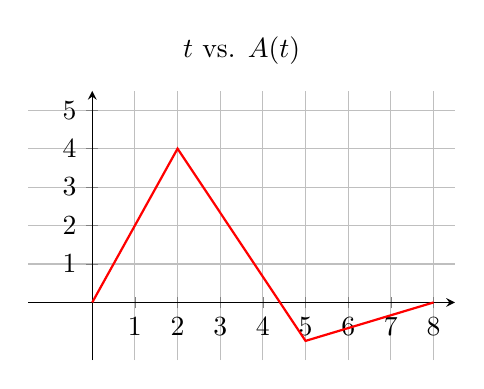
\begin{tikzpicture}
		\begin{axis}[
			title={$t$ vs. $A(t)$},
			width=7cm,
			height=5cm,
			xmin=-1.5,xmax=8.5,
			ymin=-1.5,
			ymax=5.5, xmajorgrids, ymajorgrids,
			xtick={0,...,10}, ytick={0,1,...,10},
			axis lines=middle,
			samples=5, domain=-5:5]
			
			\addplot[red, thick] coordinates {(0,0) (2,4) (5,-1) (8,0)};
		\end{axis}
	\end{tikzpicture}%
	~~~~~~~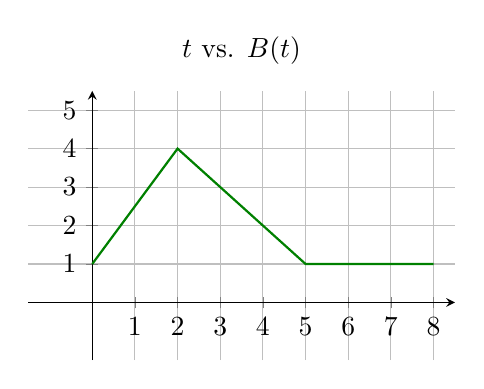
\begin{tikzpicture}
		\begin{axis}[
			title={$t$ vs. $B(t)$},
			width=7cm,
			height=5cm,
			xmin=-1.5,xmax=8.5,
			ymin=-1.5,
			ymax=5.5, xmajorgrids, ymajorgrids,
			xtick={0,...,10}, ytick={0,1,...,10},
			axis lines=middle,
			samples=5, domain=-5:5]
			
			\addplot[green!50!black, thick] coordinates {(0,1) (2,4) (5,1) (8,1)};
		\end{axis}
	\end{tikzpicture}
	\end{center}
	
	\begin{enumerate}
		\item What are the initial conditions of the graphed solution?
		\item Is the solution periodic or not? Explain.
		\item Sketch the solution in \textbf{phase space}.
	\end{enumerate}

	\item The following is a graph in \emph{phase space} of a solution to an unknown system of differential equations
	$K'(t)=\ldots$ and $L'(t)=\ldots$ with initial conditions $K(0)=0$ and $L(0)=-2$.

	\begin{center}
	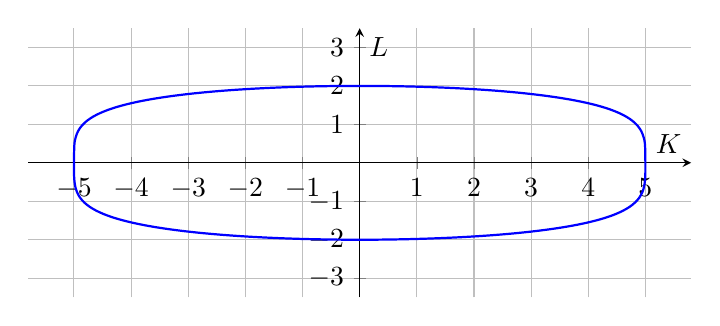
\begin{tikzpicture}
		\begin{axis}[
			width=10cm,
			height=5cm,
			xmin=-5.8,xmax=5.8,			
			ymin=-3.5,
			ymax=3.5, xmajorgrids, ymajorgrids,
			xtick={-5,...,5}, ytick={-10,...,10},
			axis lines=middle,
			samples=5, domain=-5:5,
			xlabel={$K$},
			ylabel={$L$}
			]
			
            \addplot [
                domain=0:2*pi,
                samples=100,
                smooth,
                thick,
                blue
            ] 
            ({5*sin(deg(x))}, {2*sign(cos(deg(x)))*abs(cos(deg(x)))^(1/2)});
            %({cos(deg(x)) / (1 + sin(deg(x))^2)}, {cos(deg(x)) * sin(deg(x)) / (1 + sin(deg(x))^2)});
		\end{axis}
	\end{tikzpicture}%
	\end{center}

	\begin{enumerate}
		\item Draw possible component graphs for this solution.
		\item You are given additional information: the solution curve traces out the right half 
		twice as fast as it traces out the left half.
		Draw possible component graphs based on this additional information.
	\end{enumerate}
	\item \begin{enumerate}
		\item Can you always go from component graphs to a graph in phase space? What about 
		from a graph in phase space to component graphs? Explain.
		\item List at least one benefit of (i) component graphs and (ii) graphs in phase space.
	\end{enumerate}
	
	\newpage

	% Add challenge question where the curve has a finite arc length and ask them to draw it in component space.
	\item (Challenge Question)
	The following is a graph in \emph{phase space} of a solution to an unknown system of differential equations
		$V'(t)=\ldots$ and $W'(t)=\ldots$. The solution $\Big(V(t),W(t)\Big)$ graphed below satisfies:
		(i) $V(0)=0$ and $W(0)=-2$ and (ii) $V(t)$ and $W(t)$ are defined for all $t\in \R$.

		\begin{center}
		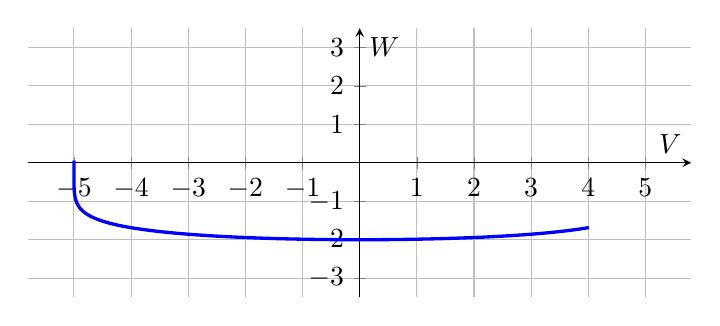
\begin{tikzpicture}
			\begin{axis}[
				width=10cm,
				height=5cm,
				xmin=-5.8,xmax=5.8,			
				ymin=-3.5,
				ymax=3.5, xmajorgrids, ymajorgrids,
				xtick={-5,...,5}, ytick={-10,...,10},
				axis lines=middle,
				samples=5, domain=-5:5,
				xlabel={$V$},
				ylabel={$W$}
				]
				
				\addplot [
					domain=(-1.5*pi+.64):(-pi/2),
					samples=100,
					smooth,
					very thick,
					blue
				] 
				({5*sin(deg(x))}, {2*sign(cos(deg(x)))*abs(cos(deg(x)))^(1/3)});
				%({cos(deg(x)) / (1 + sin(deg(x))^2)}, {cos(deg(x)) * sin(deg(x)) / (1 + sin(deg(x))^2)});
			\end{axis}
		\end{tikzpicture}%
		\end{center}

		\begin{enumerate}
			\item Draw graphs of a possible pair of $V(t)$ and $W(t)$ in \emph{component space}.
			\item The curve shown in phase space can be traced with the parametric equation \[\vec r(\theta)=\mat{5\sin\theta \\ 2{(\cos\theta)}^{1/3}}\]
			with $\theta\in(-3\pi/2 + 0.64, -\pi/2)$.

			Find a parametric equation $\vec q(t)$ so that the curve shown in phase space is traced out by $\vec q(t)$ for $t\in \R$.

			\item Come up with a system of differential equations that satisfy the conditions on $V(t)$ and $W(t)$.

			\item Come up with a second, different, system of differential equations that satisfy the conditions on $V(t)$ and $W(t)$.
		\end{enumerate}


	%\vspace{-2em}
	%\item Consider the following phase portrait of an unknown system $X'(t)=\ldots$ and $Y'(t)=\ldots$.

	%	\hspace{-1.5em}\begin{tikzpicture}[scale=.75, blue]
	%		% Define the vector field function
	%		% based on
	%		% https://www.desmos.com/calculator/o3xjzddojw
	%		% x' = (x+2.87)*y*(x+8.63)
	%		% y' = x*(y+7.23)*(y-4.27)
	%		\def\vectorfieldx(#1,#2){(#1 + 2.87) * (#2) * (#1 + 8.63) / 200}
	%		\def\vectorfieldy(#1,#2){(#1) * (#2 + 7.23) * (#2 - 4.27) / 200}

	%		% Draw the vector field
	%		\foreach \x in {-11,-10.4,...,10}
	%			\foreach \y in {-10,-9.4,...,10}
	%			{
	%				% Calculate the vector at (\x, \y)
	%				\pgfmathsetmacro\vx{\vectorfieldx(\x,\y)}
	%				\pgfmathsetmacro\vy{\vectorfieldy(\x,\y)}
	%				
	%				% Normalize the vector for consistent arrow lengths
	%				\pgfmathsetmacro\norm{sqrt(\vx*\vx + \vy*\vy + 0.01)}
	%				\pgfmathsetmacro\scaleChange{atan(\norm)/100/\norm}
	%				\pgfmathsetmacro\vx{\vx*\scaleChange}
	%				\pgfmathsetmacro\vy{\vy*\scaleChange}
	%							
	%				% Draw the vector as an arrow
	%				\draw[->] (\x,\y) -- ++(\vx,\vy);
	%			}

	%	\end{tikzpicture}
	%
	%\begin{enumerate}
	%		\item Where are the equilibrium solutions in the phase portrait? (Can you find all five?)
	%		\item Classify the nature of the equilibrium solutions as stable, unstable, attracting, repelling, etc.
	%		Give a justification for each classification.
	%		\item In phase space, the \emph{basin of attraction of an equilibrium solution $f$} is the set of initial conditions 
	%		 lead where solutions asymptotically approach $f$. For each attracting equilibrium solution, identify its basin of attraction.
	%		\item Divide the phase space into regions where solutions are:
	%		\begin{enumerate}
	%			\item Bounded vs. unbounded. 
	%			\item Periodic vs. non-periodic.
	%			\item Have horizontal asymptotes as $t\to\infty$ vs. $t\to-\infty$.
	%		\end{enumerate}	
	%		Note: when we talk about a \emph{solution}	(e.g., being bounded), we are always referring to its behaviour in component space.
	%	\end{enumerate}
	
\end{enumerate}